To complement and validate the results of the off-line evaluation, we ran a user study in our university, asking 24 students to find the natural disasters in our collection of tweets. In brief, the user study interface allows to enter a search query and then having the search results shown on an interactive map, which is used to browse the results. %The user was able to interact with the map by panning, zooming and dragging and also by clicking on tweets and clusters to get their content. 
The user was asked to find three natural disasters using a different algorithm for each trial (three algorithms to discover nine different natural disasters). At each step, the user was asked to enter information related to each natural disaster he may identify, including the type of the natural disaster, its location (US state), and the date on which he thinks the disaster happened. %In addition, we collected logs to record different behaviors and actions of the user. Moreover, each user was asked to answer a NASA TLX and a System Usability Scale surveys after each trial. Finally, at the end of the experiment, each user was asked to fill out an exit survey, which included a ranking of the algorithms.


The three different algorithms used in this user survey were: (1) a baseline method which displays all tweets that match the query (Figure \ref{Fig:GlobalDisplay}), (2) our greedy algorithm, and (3) X-Means. Note that the probability relevance score of each tweet was derived using a language model to estimate $S(j)$.
Also, for each user the sequence of algorithms to evaluate was presented differently, such that to cover all possible six combination uniformly four times (24 users). %Here we wish to indicate that the user had no indication of what algorithm was used each time, especially between the BPS and the X-Means algorithms, which both present the results in a similar way using clusters (bounding boxes). Finally, we highlight the fact that we have set up the task such that it wasn't too easy nor too difficult for the user. %On average, the experiment took 50 mn for each participate.

% Figure \ref{fig:ScreenShot} shows the interface of the user study, with the results of the query ``tornado, blizzard, earthquake''  using X-Means. The results of the same query with the baseline and the BPS algorithms are shown in Figure \ref{Fig:UseCase}.

%\begin{figure}[t]
%\begin{centering}
%{\includegraphics[width=8.5cm]{imgs/kmeans}}
%\par\end{centering}
%\caption{User survey Web page. The results of the query ``tornado, blizzard, earthquake''  are shown using clusters of X-Means, %which can be hidden/shown using the buttons at the top. The sidebar was used to provide answers.}
%\label{fig:ScreenShot}
%\end{figure}

The performance of the algorithms was measured using cumulative recall for the type and location of the natural disasters and the absolute error in the dates of the disasters starting at maximum error. The obtained results are shown in Figure \ref{fig:UserSurveyRecall} with 95\% confidence interval.
In brief, the main outcomes of this user study can be summarized as follows: 
(i) This user study confirms clearly the results obtained in the offline evaluation since the greedy algorithm outperforms K-Means and the baseline in identifying the natural disasters, their locations, and their dates.
(ii) In general, the clustering approach is clearly useful for this kind of task as both greedy and K-Means outperformed the  brute force baseline. 
(iii) Clearly, the greedy algorithm required much fewer efforts and time to complete the task than for K-Means and the baseline and that to reach a bit higher level of recall. 

 As a conclusion for this evaluation, we notice that there is a similar outcome between the two evaluation methods. Both evaluations confirm the significant contribution of the greedy algorithm for this specific relevance-driven clustering task. %Even though the off-line evaluation showed that K-Means is inappropriate for this task, the user study showed that it is effective to some extent. 
% Finally, several participants mentioned the utility, the ease and the precision provided by the greedy algorithm to complete this search task.




\begin{figure}[t]
\begin{centering}

\includegraphics[width=7.5cm]{imgs/legend9}
\par\end{centering}
\begin{centering}
{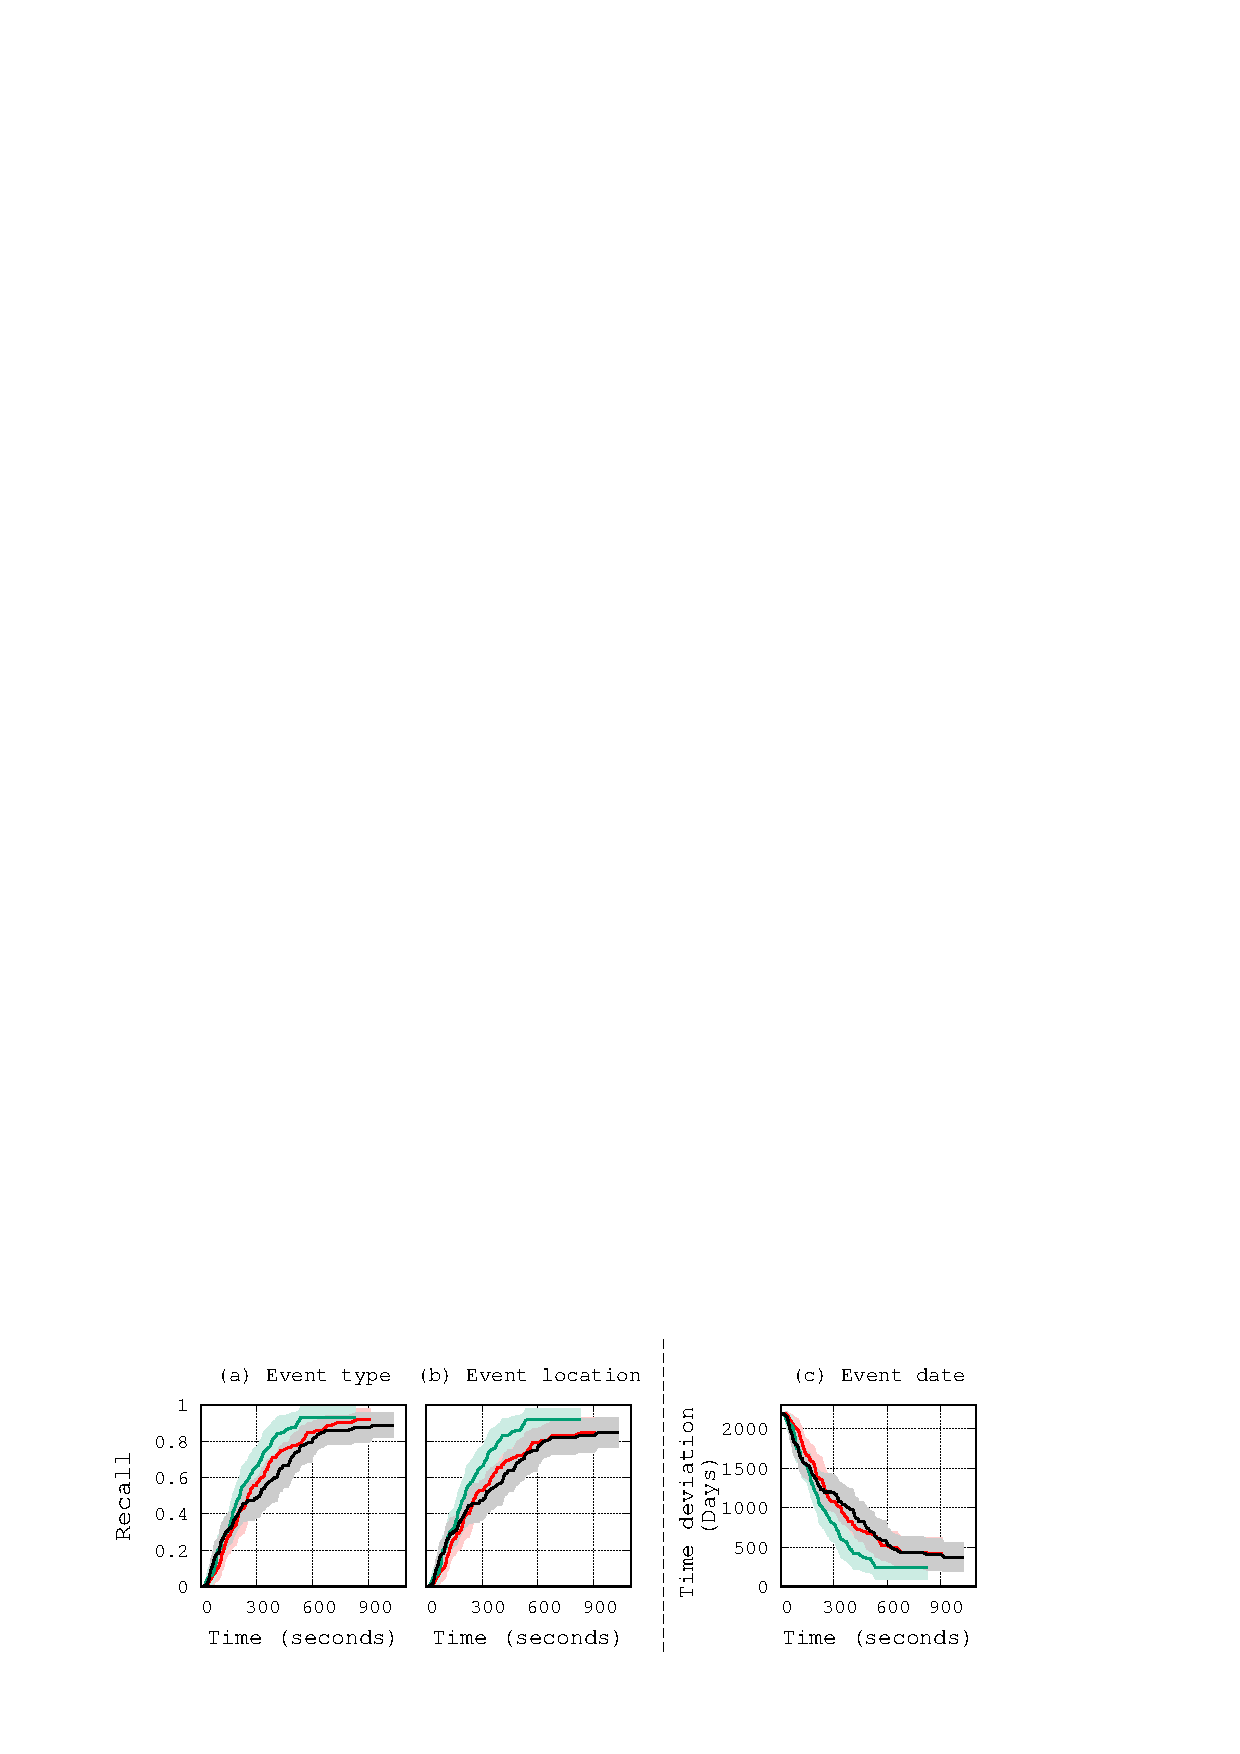
\includegraphics[width=8.5cm]{imgs/nd_recall}}
\par\end{centering}
\caption{The performance of the algorithms measured using cumulative recall for the type and location of the natural disasters and the absolute error in the dates of the disasters.}
\label{fig:UserSurveyRecall}
\end{figure}



%However, 



%\begin{figure}[t]
%\begin{centering}
%{\includegraphics[width=8cm]{imgs/ranking}}
%\par\end{centering}
%\caption{Ranking of the algorithms by participants.}
%\label{fig:UserSurveyRanking}
%\end{figure}

